\section{Algorithmen}
In der Programmierarbeit wurden mit Java schon zwei Versionen des Minimax-Algorithmus implementiert.
Eine sequenzielle (Normalfall) und eine parallele (mittels ForkJoin) Lösung.
Da die weiteren Verbesserungen in dieser Arbeit an diesen Implementierungen basieren, werden sie hier kurz dokumentiert.

\subsection{Minimax sequenziell}
\label{subsec:minimax-sequenziell}
Die sequenzielle Implementierung des Minimax-Algorithmus ist ziemlich unkompliziert.
Es besteht eine rekursive Funktion, die für jeden legalen Schachzug, bis zu einer bestimmten Tiefe, ausgeführt wird (\cite{minimaxgeeks}).
Diese Funktion implementiert die Minimax-Logik mit einer Abweichung vom Standard-Minimax-Algorithmus - sie protokolliert die Zugverläufe für jeden Zugpfad.
Dies aus zwei Gründen:
\begin{enumerate}
    \item Erleichtertes Debugging
    \item Bei Zügen mit dem gleichen Ergebnis wird der Zug mit der geringeren Tiefe, bzw.\ kürzeren Historie genommen
\end{enumerate}

Zusätzlich besteht eine vorzeitige Rückgabe bei Zug-Pfaden, welche zum Schluss vom Spiel führen (z.B.\ Schachmatt). \\
Beispiel: Die angegebene Tiefe ist 5, jedoch wird mit einer bestimmten Zugkombination nach 3 Zügen Schachmatt erzeugt - somit rechnet die Funktion nur bis zur Tiefe 3.

\begin{figure}[H]
    \centering
    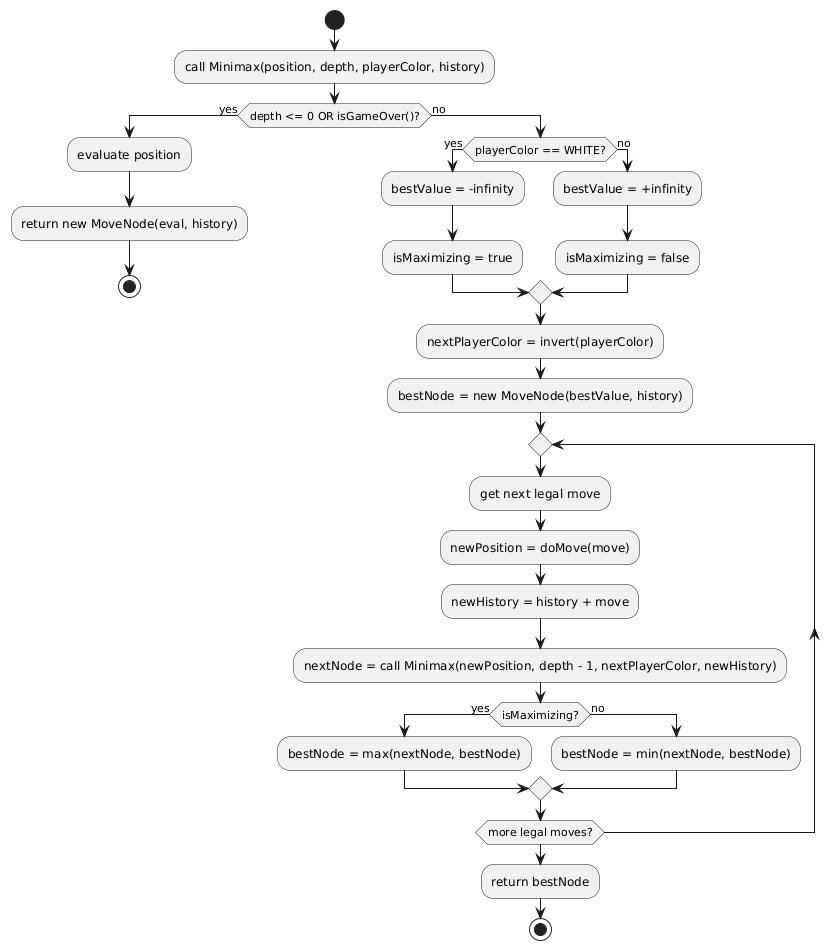
\includegraphics[width=\linewidth]{generated-diagrams/sequential-minimax}
    \caption{Ablaufdiagramm - Minimax sequenziell}
    \label{fig:minimax-sequential}
\end{figure}

Die Umsetzung sieht im Code folgendermassen aus:
\lstinputlisting[
    firstline=28,
    lastline=57,
    firstnumber=28,
    caption={Minimax sequenziell},
    label={lst:minimax-sequenziell}
]{../src/main/java/ch/hslu/cas/msed/blobfish/minimax/MiniMaxSequential.java}

\subsection{Minimax parallel}
\label{subsec:real-minimax-parallel}
Die parallele Implementierung enthält die gleiche Basislogik, jedoch wird anstelle einer Iteration für alle legalen Züge das ForkJoin Prinzip verwendet.
Für jeden legalen Zug wird ein Task erstellt.
Alle erstellten Tasks werden zur Ausführung zum ForkJoin Pool hinzugefügt.
Dies passiert rekursiv für jede Tiefe.
Anschliessend wird gewartet bis alle Tasks einer bestimmten Tiefe fertig sind und die Resultate der Ergebnisse werden durch die Minimax-Logik überprüft.

\begin{figure}[H]
    \centering
    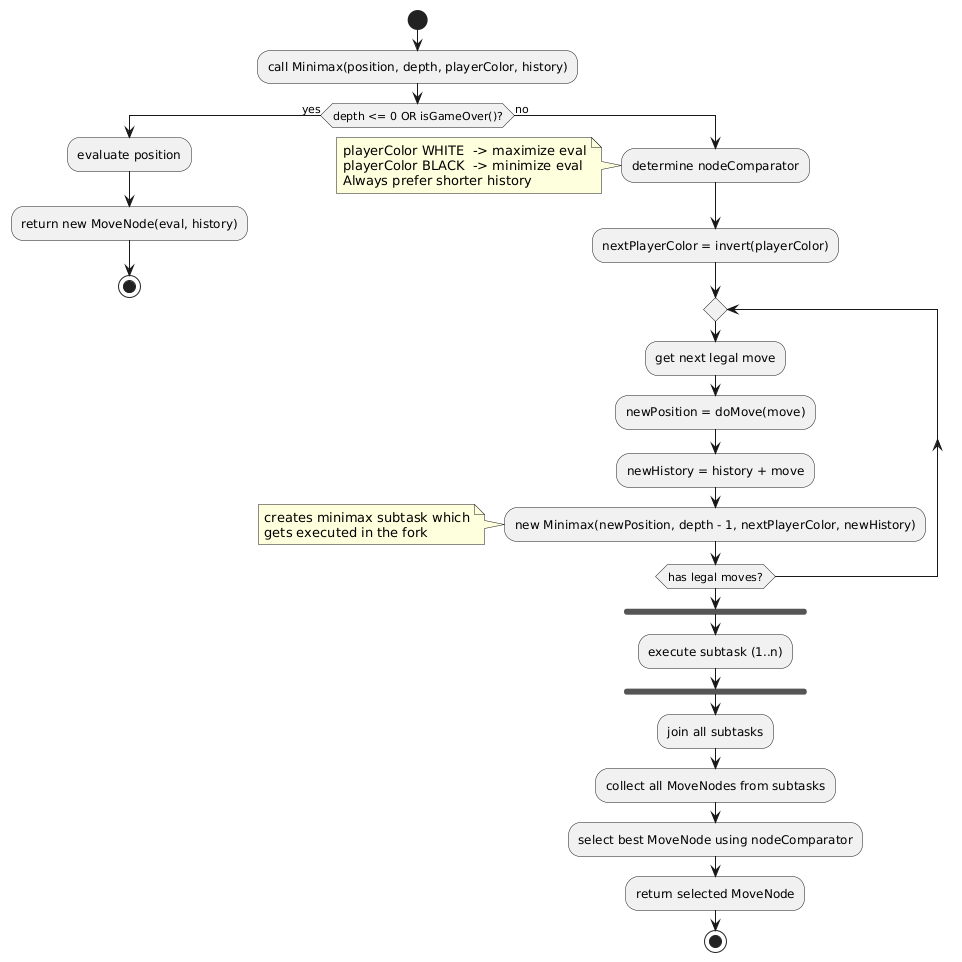
\includegraphics[width=\linewidth]{generated-diagrams/forkjoin-minimax}
    \caption{Ablaufdiagramm - Minimax parallel}
    \label{fig:minimax-parallel}
\end{figure}

Jeder Task führt die \texttt{compute}-Methode aus.
Der folgende Code-Abschnitt zeigt die Hauptlogik der \texttt{MiniMaxRecursiveTask} Klasse, bzw.\ die \texttt{compute}-Methode.
\lstinputlisting[
    firstline=33,
    lastline=53,
    firstnumber=33,
    caption={Minimax ForkJoin Task - compute Methode},
    label={lst:minimax-forkjoin-task-compute}
]{../src/main/java/ch/hslu/cas/msed/blobfish/minimax/base/MiniMaxRecursiveTask.java}

Die Threshold-Logik in dieser Methode wurde nachträglich in dieser Arbeit implementiert, laut Dozentenfeedback aus der Programmierarbeit.
Bei einer kleinen Anzahl an legalen Zügen ist der Overhead zur Threaderstellung grösser als der Geschwindigkeitsgewinn.
Ähnlich werden bei einer grossen Zugtiefe schon viele Threads erstellt und das Erstellen von weiteren Threads führt zu einem Overhead.
Die Einführung des Thresholds sorgt dafür, dass in diesen Situationen die Schachzüge sequenziell, bzw.\ im gleichen Thread evaluiert werden.

Im Code-Abschnitt~\ref{lst:minimax-forkjoin-task-subtask-erstellung} ist die Erstellung neuer Tasks ersichtlich.
\lstinputlisting[
    firstline=71,
    lastline=80,
    firstnumber=71,
    caption={Minimax ForkJoin Task - Sub-Task Erstellung},
    label={lst:minimax-forkjoin-task-subtask-erstellung}
]{../src/main/java/ch/hslu/cas/msed/blobfish/minimax/base/MiniMaxRecursiveTask.java}

Die Erstellung des ersten Tasks befindet sich in der Klasse \texttt{MiniMaxParallel}.
Dieser Task wird über den ForkJoin \texttt{commonPool} ausgeführt.
\lstinputlisting[
    firstline=26,
    lastline=34,
    firstnumber=26,
    caption={Minimax parallel Task-Aufruf},
    label={lst:minimax-parallel}
]{../src/main/java/ch/hslu/cas/msed/blobfish/minimax/MiniMaxParallel.java}